\documentclass[11pt, oneside]{article}   	% use "amsart" instead of "article" for AMSLaTeX format
\usepackage{geometry}                		% See geometry.pdf to learn the layout options. There are lots.
\geometry{letterpaper}                   		% ... or a4paper or a5paper or ... 
%\geometry{landscape}                		% Activate for rotated page geometry
%\usepackage[parfill]{parskip}    		% Activate to begin paragraphs with an empty line rather than an indent
\usepackage{graphicx}				% Use pdf, png, jpg, or eps§ with pdflatex; use eps in DVI mode
								% TeX will automatically convert eps --> pdf in pdflatex		
\usepackage{amssymb}

\usepackage{outlines}

%SetFonts

%SetFonts


\title{A Search for  Extended Circumgalactic Dust}
\author{Jacqueline McCleary \& Eric Huff}
%\date{}							% Activate to display a given date or no date

\begin{document}
\maketitle
%\section{}
%\subsection{}

% OK so what the fuck do I want to put in here? I guess it makes sense to start by putting in the figures that I want to put in
% Those would include: the dusty dust figure, the star-fg correlation, the fg/bkg samples, what else? I guess the Galex and IIFSC plots? I'm much less
% convinced by those, but I guess we can start... Also, the spatial correlation function would be good. 

\section{Motivation\label{sec:intro}}
\begin{outline}
\1 Motivate the research based on literature results: obviously Menard, but also Peek, and the theory papers. Do not include figures, except maybe in an appendix
\1 DO NOT CONGRATULATE
\1 Should probably explain how Av, reddening and Rv are related to one another
\2 Linearly related! But dust-model dependent
\2 We chose Rv = 3.1 as a default, but others may be better...
\3 consider moving this discussion to methods?
\end{outline}


\section{Methods\label{sec:methods}}

\subsection{A Maximum Likelihood Estimator for Dust Extinction}
\begin{outline}
\1 Develop our MLE formalism; reproduce equations
	\2 don't forget to include discussion of extinction vector (FM07 or whatever)
\1 May also want to include the ON and optimal vector generation, at least for a paragraph --YES
	\2 Think of this like a PCA; as long as the sum is non-negative, we're in good shape. 
	\2 Dips positive or negative mean that the``principal component" under or overfits the actual trend at that distance
		\3 little harder to connect to physical meaning for now -- problem for theorists?
	\2 For development of "optimal" vector, mb show chi-squared plots, just to explain where we got this? 
		\3 I think I baleeted those, but fairly easy to reproduce 
\1 Discuss how and why we split Av estimate into redshift bins
	\2 correlating *deviations from mean color space of background galaxies*
	\2 \textbf{HEY: did we deredden our magnitudes for galactic reddening? Are we hoping that we just "average" over dust? Because that's a bad idea}
\1 \textbf{yooo need to justify $R_V = 3.1$ and consider using other values of $R_V$}
\end{outline}

\subsection{Correlation Function Algorithm\label{ssec:treecorr}}
\begin{outline}
\1 Treecorr algorithm, briefly: it's not my algorithm but it is what we use. Correlating not gal-shear but gal-extinction
\1 Mention spatial correlation as well
\1 Mention null tests: flexibility of algorithm allows us to easily correlate any two samples, so ideal for null tests like star-extinction
\end{outline}

\section{Datasets}\label{sec:data}

\begin{outline}
\1 Discuss samples that we used: 
	\2 redMaGiC as background (discuss algorithm, add some plots of color variance with MLE or color-color plots)
		\3 area covers: $290\degree \lesssim \alpha \lesssim 110\degree$
	\2 GALEX and IIFSCz (maybe) 
\1 Also SVM for DES foreground sample 
	\2 give some characteristics
	\2 perhaps move discussion of algorithm to \ref{sec:methods}
		\3 ref needed
\1 Might be good to have some consistency plots showing overlap of two samples
\1 Used Healpy to ensure that we are not correlating across empty space, which would have the effect of diluting the observed signal
\end{outline}

\begin{figure}[htbp] %  figure placement: here, top, bottom, or page
   \centering
   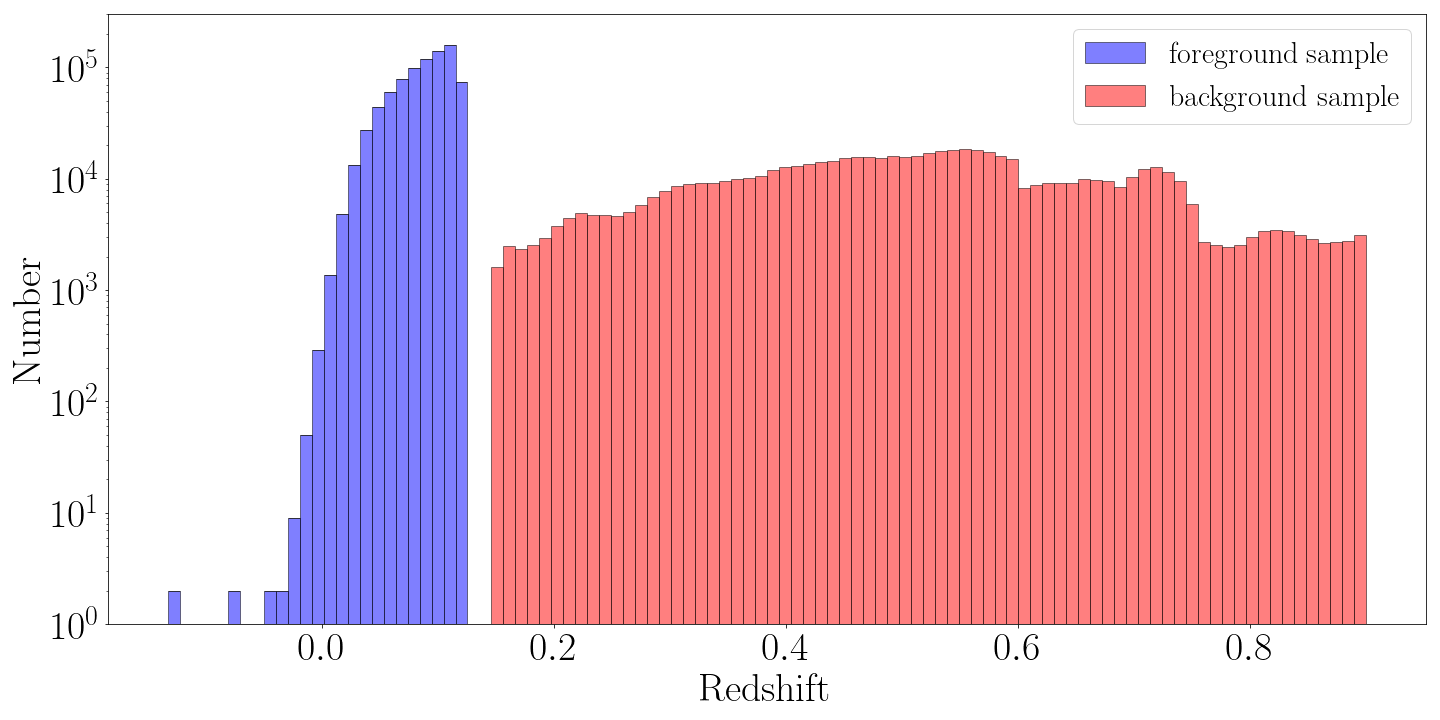
\includegraphics[width=0.75\textwidth]{figures/redshift_histograms.png} 
	\caption{Redshift distribution of foreground and background samples}
   \label{fig:redshifts}
\end{figure}

\section{Results\label{sec:results}}
\begin{outline}
\1 Plot up all the results I do have... with dust vector, "optimal" vector for all samples 
\1 MB show the "dust mass plot" but maybe also skip because it's not really a dust mass
\1 Star-bkg correlation is a good null test to show 
\end{outline}

\section{Conclusions\label{sec:conclusions}}
\begin{outline}

\1 Start discussing consequences: here, compare to literature
\1 It might be cool to compare to MgII absorption plot, since that also shows evidence for extinction
	\2 Except that maybe that's controversial for actual MgII folks? Apparently they expect this to be anti-correlated
\1 For the literature figures, consider placing in appendix?
\end{outline}

\end{document}  